\documentclass[a4paper,10pt]{article}
\usepackage[utf8]{inputenc}
\usepackage[T1]{fontenc}
\usepackage[french]{babel}
\frenchbsetup{StandardLists=true} % à inclure si on utilise \usepackage[french]{babel}
\usepackage{enumitem}
\usepackage{amssymb}
\usepackage{graphicx}
% Title Page
\title{Rapport gestion de l'hotel}
\author{
  Romain PEREIRA\\
  \newline
  Douha ORHIMI\\
  \and
  Laurie PANDRAUD\\
  \newline
  Yi LU\\
}
\date{Dimanche 10 Décembre 2017}

\usepackage{hyperref}
\hypersetup{
    colorlinks,
    citecolor=black,
    filecolor=black,
    linkcolor=blue,
    urlcolor=black
}


\begin{document}
\maketitle
\tableofcontents

  \section{Préambule}
    Autrefois dis 'le Bien-heureux', notre équipe a repris en main la gestion du nouvel hotel 'Ocre'. La précèdente équipe l'a laissé dans un état négligé.
    Notre objectif est de gérer l'hôtel de manière économiquement viable pendant ces 4 prochaines années, partagées en semestres de hautes et basses saisons.
    \newline
    \newline
    L’hôtel Ocre s’établit dans un contexte de concurrence avec 6 autres établissements qui partent d’une situation économique similaire.
    L’hôtel a initialement une capacité d’accueil de 50 chambres qui ont été gérées par 4 employés permanents et 2 employés temporaires.
    \newline
  \newpage
  \section{Stratégie de developpement : domestique}
    \subsection{Tour 1 : 1er hiver}
      Nous avons recuperé l'hotel en basse saison.
    \subsection{Tour 2 - Tour 3}
      • 2 permanents à l'international (2400 chambres possibles sur les 3600 théoriques... economie là dessus ou un 3eme temporaire?)
      • reduction prix domestique pour ecraser concurrence
      • recrutement 1 permanent et de 2 temporaires pour l'été
      • "4000 euros par employé à 6000 euros cette année et on s'attend à des augmentations sur le même rythme à l'avenir." => embaucher maintenant
      • dette, que fais ton? empruntes pour plus de chambre? economise pour focus international?
      • marketting du dernier tour faible par rapport aux autres, mais ce ressent peu au niveau des resultats... apres c'etait l'hiver



    \subsection{Tour 5 - Tour 8}
     
   \newpage
   \section{Stratégie de developpement : international}
    
    \subsection{Tour 1 - Tour 2}
      Notre équipe a decidé de s'implanter à l'international dés le 1er tour.
      \newline
      Notre stratégie globale à long terme était de louer beaucoup de chambres, et peu chère. En s'assurant de faibles marges,
      sur les 1ères saisons, on esperait tuer la concurrence et obtenir le monopole du marché sur le long terme.
      \newline
      \newline
      Le 1er hiver, nous decidons donc de louer 20 chambres (le maximum possible) pour la prochaine haute saison.
      \newline
      \newline
      Arrivé à l'été, les conditions de marchés indiquent que la demande internationale a une bonne dynamique.
      Ayant recuperé les locaux dans un parfait état, et voyant que nos concurrents ont peu de chambres sur le marché international,
      nous optons pour une politique de prix élevés (~ 140€), en esperant que l'offre sature par rapport à la demande.
      Notre politique de marketting est défensive: nous nous alignons sur nos concurrents, afin de limiter les frais.
      \newline
      Ces choix n'ont pas été efficace: nos locaux sont seulement occupés à 73\%, alors que nos concurrents retombent eux plus facilement sur les frais.
      Nous avons pris note de cette erreur et ajusterons nos prix pour les prochaines saisons.
      \newline
      \newline
      Convaincu par notre stratégie, nous prenons 10 chambres de plus, pour un total de 30 chambres pour le prochain hiver.
      \newline
      Les faibles résultats de cette saison hivernale s'explique par cette investissement.
    \subsection{Tour 3 - Tour 8}
      Le marché international ne connait finalement pas l'essor attendu. L'épisode de grippe aviaire au 2ème été a détruit le marché.
      Nous ne prenons donc pas de chambres supplémentaires, et rentabilisons au mieux nos chambres. (peu de renovations, optimisations des charges du personnels).
      \newline
      En limitant ainsi les risques à l'international, nous concentrons nos investissements sur le marché domestique.
      \newline
      \newline
      Le marché reprends de la dynamique au dernier été. Grâce à notre politique de prix bas, nous obtenons la plus grosse part du marché, en se plaçant nettement devant
      'La Rose' 'Hotel Aviv', qui sont nos concurrents directes. Nous esperons ainsi les essoufler et croître plus vite qu'eux.

  \newpage
  \section{Perspectives futures et conclusion}
    hello world
    
  \newpage
  \section{Graphiques, chiffres...}
    Ces quelques graphiques illustrent nos propos. Nous comparons ici nos données avec nos 2 principaux concurrents.
    \newline
        
    \begin{figure}[!h]
      \begin{center}
	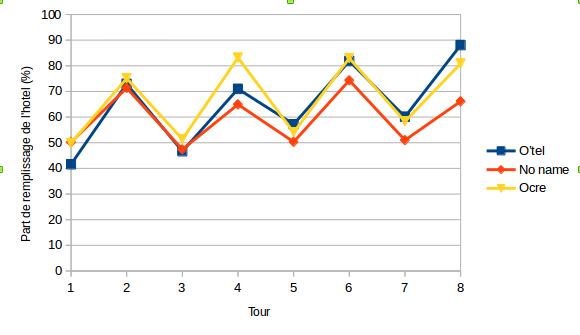
\includegraphics[height=7cm,keepaspectratio]{./images/remplissage_hotel.png}
      \end{center}
      \caption{\textit{Remplissage de l'hotel (domestique)}}
    \end{figure}
    
    \begin{figure}[!h]
      \begin{center}
	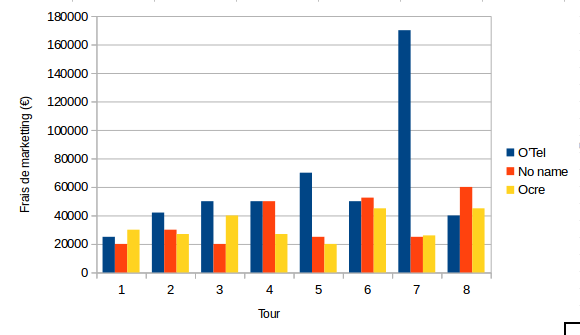
\includegraphics[height=7cm,keepaspectratio]{./images/frais_marketting.png}
      \end{center}
      \caption{\textit{Frais marketting}}
    \end{figure}
    
    \begin{figure}[!h]
      \begin{center}
	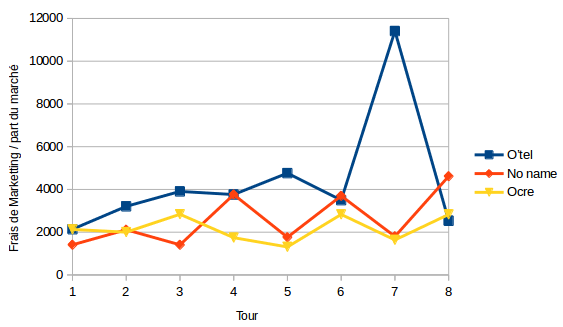
\includegraphics[height=7cm,keepaspectratio]{./images/marketting_part_marche.png}
      \end{center}
      \caption{\textit{Remplissage de l'hotel en fonction des frais de marketting (domestique)}}
    \end{figure}
    
    \begin{figure}[!h]
      \begin{center}
	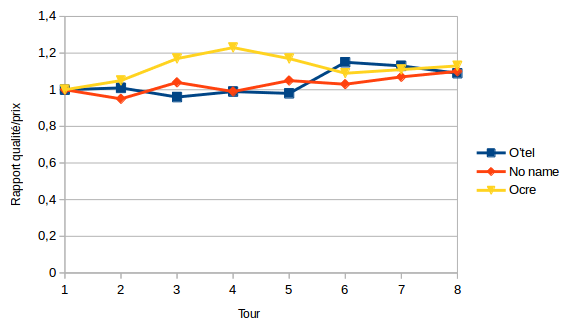
\includegraphics[height=7cm,keepaspectratio]{./images/rapport_qualite_prix.png}
      \end{center}
      \caption{\textit{Rapport qualité/prix (domestique)}}
    \end{figure}

    \begin{figure}[!h]
      \begin{center}
	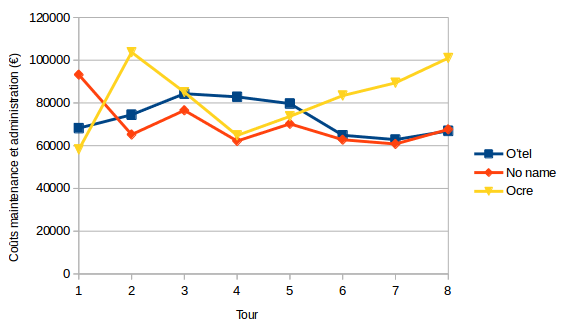
\includegraphics[height=7cm,keepaspectratio]{./images/cout_administration_et_maintenance.png}
      \end{center}
      \caption{\textit{Coût d'administration et de maintenance (domestique)}}
    \end{figure}

    
    \begin{figure}[!h]
      \begin{center}
	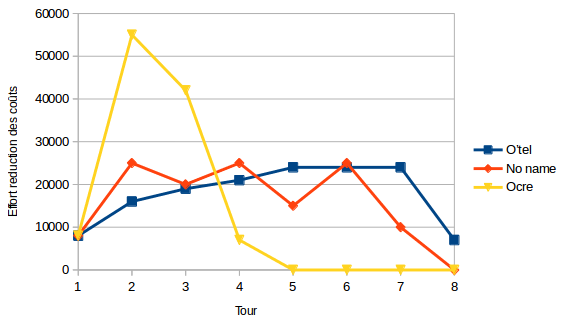
\includegraphics[height=7cm,keepaspectratio]{./images/effort_reduction_couts.png}
      \end{center}
      \caption{\textit{Effort reductions des coûts (domestique)}}
    \end{figure}
    
\end{document}          
